\subsection{Convergence results for Gradient Descent}
\begin{itemize}
    \item Lipschitz-convex functions: $O\left(\dfrac{1}{\epsilon^2}\right)$
    \item Smooth functions: $O\left(\dfrac{1}{\epsilon}\right)$
    \item Smooth and strongy convex functions: $O\left(\dfrac{1}{\log(\epsilon)}\right)$
    \item Accelerated gradient descent: $O\left(\dfrac{1}{\sqrt{\epsilon}}\right)$
\end{itemize}

\subsection{Accelerated Gradient Descent}
Aim: minimizing convex function $f: \mathbb{R}^d \to \mathbb{R}$ (with gradient $\nabla f$). "First order method" because it only uses the function and its gradient. What is the best first order method?\\
Nemirovski and Yudin (1979): every first order method needs in the worst case $O\left(\dfrac{1}{\sqrt{\epsilon}}\right)$ steps. \\
Nesterov (1983): accelerated gradient descent (AGD). Let $f: \mathbb{R}^d \to \mathbb{R}$ convex, differentiable and smooth with parameter $L$. ADG reads:
\begin{itemize}
    \item choose $\underline{z}^{(0)} = \underline{y}^{(0)} = \underline{x}^{(0)}$
    \item for $k \geq 0$ set:
    \begin{itemize}
        \item $\underline{y}^{(k+1)} = \underline{x}^{(k)} - \dfrac{1}{L} \nabla f(\underline{x}^{(k)})$ \hspace{2cm} Normal step
        \item $\underline{z}^{(k+1)} = \underline{z}^{(k)} - \dfrac{k+1}{2L} \nabla f (\underline{x}^{(k)})$ \hspace{2cm} Aggressive step
        \item $\underline{x}^{(k+1)} = \dfrac{k+1}{k+3} \underline{y}^{(k+1)} + \dfrac{2}{k+3} \underline{z}^{(k+1)}$ \hspace{2cm} Average 
    \end{itemize}
\end{itemize}

\textbf{Theorem of convergence of AGD}: lef $f: \mathbb{R}^d \to \mathbb{R}$ convex, differentiable with a global minimum $\underline{x}^*$ and smooth with parameter $L$. AGD yields:
\[
f(\underline{y}^{(N)}) - f(\underline{x}^*) \leq \dfrac{2L \Vert \underline{z}^{(0)} - \underline{x}^* \Vert^2}{N(N+1)}  \hspace{1cm} N > 0   
\]
\textbf{Definition of smooth and strongly convex functions}: Let $f: \text{dom}(f) \to \mathbb{R}$ be a convex and differentiable function, $X \subseteq \text{dom}(f)$ convex and $\mu \in \mathbb{R}^+$. Function $f$ is called strongly convex with parameter $\mu$ over $X$ if:
\[
f(\underline{y}) \geq f(\underline{x}) + \nabla f(\underline{x})^T (\underline{y} - \underline{x}) + \dfrac{\mu}{2} \Vert \underline{y} - \underline{x} \Vert^2 \hspace{1cm} \forall \underline{x}, \underline{y} \in X    
\] 
Remark
\begin{itemize}
    \item \textbf{smoothness}: $\forall \underline{x} \in X$ the graph of $f$ is below a not-too-steep tangent paraboloid.
    \item \textbf{Strongly-convex}: $\forall \underline{x} \in X$ the graph of $f$ is above a not-too-flat tangent paraboloid.\\ 
\end{itemize}

Theorem of convergence: strongly convex case: let $f: \mathbb{R}^d \to \mathbb{R}$ be a convex, differentiable. Suppose that $f$ is smooth with parameter $L$ and strongly convex with parameter $\mu$ > 0. Choosing:
\[
    \nu = \dfrac{1}{L}    
\]
Gradient Descent with arbitrary initial point $\underline{x}^{(0)}$ satisfies:
\begin{enumerate}
    \item Squared distances to $\underline{x}^*$ are geometrically decreasing: $\Vert \underline{x}^{(k+1)} - \underline{x}^* \Vert^2 \leq \left(1-\dfrac{\mu}{L}\right)\Vert \underline{x}^{(k)} - \underline{x}^* \Vert$ \hspace{1cm} $k \geq 0$
    \item Absolute error after N iterations is exponentially small in N: $f(\underline{x}^{(N)}) - f(\underline{x}^*) \leq \dfrac{L}{2}\left(1-\dfrac{\mu}{L}\right)^N \Vert \underline{x}^{(0)} - \underline{x}^* \Vert^2$ \hspace{1cm} $N > 0$
\end{enumerate}
Remember: recalling that $\ln(1+x)\leq x$ we have:
\[
    N \geq \dfrac{L}{\mu} \ln\left(\dfrac{R^2 L}{2\epsilon}\right)    
\]

\section{How a neural network works}
Let's define some quantities:
\begin{itemize}
    \item $w_{jk}^l$ = weight from k-th neuron in layer ($l-1$)-th to $j$-th neuron in layer $l$-th
    \item $b_j^l$ = bias of $j$-th neuron in layer $l$-th
    \item $a_j^l$ = activation of $j$-th neuron in layer $l$-th
\end{itemize}
In particular:
\[
    a_j^l = \sigma\left(\sum_{k=1}^{n_{l-1}} w_{jk}^l a_k^{l-1} + b_j^l\right)    
\]
Or in matrix form:
\[
    \underline{a}^l = \underbrace{\sigma(W^l \underline{a}^{l-1} + \underline{b}^l)}_{\underline{z}^l}
\]
where $\underline{W}^l$ is the matrix of weights (the elements are given by $W^l(j,k) = w_{jk}^l$), $\underline{b}^l$ is the vector of biases and $\underline{z}^l$ is the vector of activations.\\
The sum in the first equation above refers to the neurons in the previous layer (so $l-1$).

\subsection{Cost function J}
The aim is to compute $\frac{\partial J}{\partial w}$ and $\frac{\partial J}{\partial b}$ with backpropagation for each $w$ and $b$ in the network.
\begin{enumerate}
    \item The cost function can be written as an average over the cost functions for each sample:
    \[
        J = \dfrac{1}{N} \sum_n J_n    
    \]
    For example $J_n = \frac{1}{2}\Vert y_n - \bar{y}_n \Vert^2, \bar{y}_n = a_n^L$.
    \item The function can be written in terms of the outputs of the neural network:
    \[
        J = J(\underline{a}^L)    
    \]
\end{enumerate}

\subsection{Fundamental relations}
We define a new quantity:
\[
    \delta_j^l = \dfrac{\partial J}{\partial z_j^l}    
\]
The term $\delta_j^l$ is the error in the $j$-th neuron in the $l$-th layer so with the notation $\underline{\delta}^l$ we mean the vector of errors in the $l$-th layer.\\

Now we can write the fundamental relations:
\begin{enumerate}
    \item Error in output layer $\delta^L$
    \[
        \delta_j^L = \dfrac{\partial J}{\partial a_j^L} \sigma'(z_j^L) \hspace{1cm} \underline{\delta}^L = \nabla_a J \odot \sigma'(\underline{z}^L)    
    \]
    Check footnote about the mathematical symbol $\odot$\footnote[1]{The symbol $\odot$ means element-wise multiplication (Hadamard product) and from now on we will be using it instead of $\cdot^*$ that was used in the previous notes.}. Here is the proof:
    \[
        \delta_j^L = \dfrac{\partial J}{\partial z_j^L} = \sum_k \dfrac{\partial J}{\partial a_k^L} \dfrac{\partial a_k^L}{\partial z_j^L} 
    \]
    The sum is over all the neurons in the output layer (layer L). $a_k^L$ of the k-th neuron depends only on $z_j^L$ for the j-th neuron when $k=j$, so:
    \[
        \dfrac{\partial a_k^L}{\partial z_j^L} = 0 \hspace{0.1cm} \text{for} \hspace{0.1cm} k\neq j \implies \delta_j^L = \dfrac{\partial J}{\partial a_j^L} \dfrac{\partial a_j^L}{\partial z_j^L} = \dfrac{\partial J}{\partial a_j^L} \sigma'(z_j^L)    \hspace{0.3cm} \left(a_j^L = \sigma(z_j^L)\right)
    \]
    \item Error $\underline{\delta}^l$ in terms of error in next layer $\underline{\delta}^{l+1}$
    \[
        \underline{\delta}^l = \left[(W^{l+1})^T \underline{\delta}^{l+1}\right] \odot \sigma'(\underline{z}^l)    
    \]
    Proof:
    \[
        \delta_j^l = \dfrac{\partial J}{\partial z_j^l} = \sum_k \dfrac{\partial J}{\partial z_k^{l+1}} \dfrac{\partial z_k^{l+1}}{\partial z_j^l} = \sum_k  \delta_k^{l+1}  \dfrac{\partial z_k^{l+1}}{\partial z_k^l}
    \]
    But
    \[
        \begin{split}
            &\underset{\Big{\Downarrow} }{z_k^{l+1}} = \sum_j w_{kj}^{l+1} a_j^l + b_k^{l+1} = \sum_j w_{kj}^{l+1} \sigma(z_j^l) + b_k^{l+1} \\
            &\dfrac{\partial z_k^{l+1}}{\partial z_k^l} = w_{kj}^{l+1} \sigma'(z_j^l) \implies \delta_j^l = \sum_k w_{kj}^{l+1} \delta_k^{l+1} \sigma'(z_j^l)\\
        \end{split}
    \]
    \item Variation of cost function $J$ with respect to bias
    \[
        \dfrac{\partial J}{\partial b_j^l} = \delta_j^l
    \]
    Proof:
    \[
        \dfrac{\partial J}{\partial b_j^l} = \dfrac{\partial J}{\partial z_j^l} \dfrac{\partial z_j^l}{\partial b_j^l} 
    \]
    \[
        z_j^l = \sum_k w_{jk}^l a_k^{l-1} + b_j^l \implies \dfrac{\partial z_j^l}{\partial b_j^l} = 1 \implies \dfrac{\partial J}{\partial b_j^l} = \delta_j^l    
    \]
    \item Variation of cost function $J$ with respect to weight
    \[
        \dfrac{\partial J}{\partial w_{jk}^l} = a_k^{l-1} \delta_j^l
    \]
    Proof:
    \[
        \dfrac{\partial J}{\partial w_{jk}^l} = \underbrace{\dfrac{\partial J}{\partial z_j^l}}_{\delta_j^l} \underbrace{\dfrac{\partial z_j^l}{\partial w_{jk}^l}}_{a_k^{l-1}} = \delta_j^l a_k^{l-1}
    \]
\end{enumerate}
\textbf{Summary of the fundamental relations}:
\begin{enumerate}
    \item $\delta_j^L = \dfrac{\partial J}{\partial a_j^L} \sigma'(z_j^L) \hspace{1cm} \underline{\delta}^L = \nabla_a J \odot \sigma'(\underline{z}^L)$
    \item $\underline{\delta}^l = \left[(W^{l+1})^T \underline{\delta}^{l+1}\right] \odot \sigma'(\underline{z}^l)$
    \item $\dfrac{\partial J}{\partial b_j^l} = \delta_j^l$
    \item $\dfrac{\partial J}{\partial w_{jk}^l} = a_k^{l-1} \delta_j^l$
\end{enumerate}
\textbf{Remark}: in 2, the matrix $(W^{l+1})^T$ is the transpose of the matrix of weights of the next layer and backpropagates the error, With 1 and 2 we can compute $\underline{\delta}^l$ for all layers.\\

\noindent\textbf{Remark}: the $\underline{z}^l$ and $\underline{z}^L$ are computed in the forward procedure.\\

\noindent\textbf{Remark}: if $a_k^{l-1}$ is small in 4, then $\dfrac{\partial J}{\partial w_{jk}^l}$ is small. This means that the weight $w_{jk}^l$ is not updated much and the neural network will learn slowly.\\

\noindent\textbf{Remark}: in 1 we have $\sigma'(\underline{z}^L)$. If we use the sigmoid then for $z \to \pm \infty$ the function tends to 1 or 0 respectively and it is flat, hence in those situations we have $\sigma'(\underline{z}^L) \approx 0$. So in the last layer if the activation is high ($\approx 1$) or low ($\approx 0$) then the neuron will learn slowly (the neuron has \textbf{saturated}). Similarly for the biases.


\subsection{Algorithm}
\begin{enumerate}
    \item $\underline{x}$ input vector $\to$ compute $\underline{a}^1$ (input layer)
    \item Feedforward: for each $l=2,3,...,L$ compute $\underline{z}^l$ and $\underline{a}^l$:
    \[
        \underline{z}^l = W^l \underline{a}^{l-1} + \underline{b}^l \hspace{1cm} \underline{a}^l = \sigma(\underline{z}^l)     
    \] 
    \item Output error $\underline{\delta}^L$, compute it as:
    \[
        \underline{\delta}^L = \nabla_a J \odot \sigma'(\underline{z}^L)    
    \]
    \item Backpropagate the error: for each $l=L-1, L-2, ..., 2$ compute $\underline{\delta}^l$:
    \[
        \underline{\delta}^l = \left[(W^{l+1})^T \underline{\delta}^{l+1}\right] \odot \sigma'(\underline{z}^l)
    \]
    \item Output values of the derivatives. Compute:
    \[
        \dfrac{\partial J}{\partial b_j^l} = \delta_j^l \hspace{1cm} \dfrac{\partial J}{\partial w_{jk}^l} = a_k^{l-1} \delta_j^l
    \]
\end{enumerate}

\subsection{Stochastic Gradient Descent (SGD)}
Find $w^* = \arg\min_{\underline{w}} J(\underline{w})$. Until now we have considered the standard gradient descent for which the iterations where given by $\underline{w}^{(k+1)} = \underline{w}^{(k)} - \eta \nabla J(\underline{w}^{(k)})$. We can define the finite sum of $J$ as $J(\underline{w}) = \dfrac{1}{N} \sum_{i=1}^{N} J_i(\underline{w})$ where $N$ is the number of samples.

For example: $J(\underline{w}) = \dfrac{1}{N}\Vert \underline{y} - X\underline{w}\Vert^2 = \dfrac{1}{N} \sum_{i=1}^N \underbrace{\left(y_i - \underline{x}_i^\intercal \underline{w}\right)^2}_{J_i}$ (LS). \\

The stochastic gradient descent method at iteration $k$, select a random sample $i_k \in \{1,2,\dots,N\}$ and update the weights as:
\[
    \underline{w}^{(k+1)} = \underline{w}^{(k)} - \eta \nabla J_{i_k}(\underline{w}^{(k)})
\]
Where $J_{i_k}$ is the cost function for the $i_k$-th sample. The important thing is that the gradient descent is computer \textbf{for only one sample at a time so this results in being N times faster than the standard GD!}.

Remark: in ML we have training data $\{(\underline{x}_1, y_1), \dots, (\underline{x}_N, y_N)\}$ where $\underline{x}_i \in \mathbb{R}^d$, both $N$ and $d$ are large. \\

\textbf{1D example}.\\
We have:
\[
    J(w) = \dfrac{1}{2}\sum_{i=1}^N \left(x_i w - b_i\right)^2   
\]
Each $\left(x_i w - b_i\right)^2$ is a quadratic function. I want to minimize each $J_i$ so i set the derivative to zero:
\[
    \dfrac{\partial J_i}{\partial w} = 0 \implies \dfrac{1}{2}2\left(x_i w - b_i\right)x_i = 0 \implies w = \dfrac{b_i}{x_i}
\]
For the whole function we have:
\[
    \dfrac{\partial J}{\partial w} = \sum_{i=1}^N \dfrac{\partial J_i}{\partial w} = \sum_{i=1}^N \left(x_i w - b_i\right)x_i = 0 \implies \underline{w}^* = \dfrac{\sum_{i=1}^N b_i x_i}{\sum_{i=1}^N x_i^2}    
\]
\[
  w^* \in \left[\min_i \dfrac{b_i}{x_i}, \max_i \dfrac{b_i}{x_i}\right]  
\]
We can plot it as:
\begin{center}
    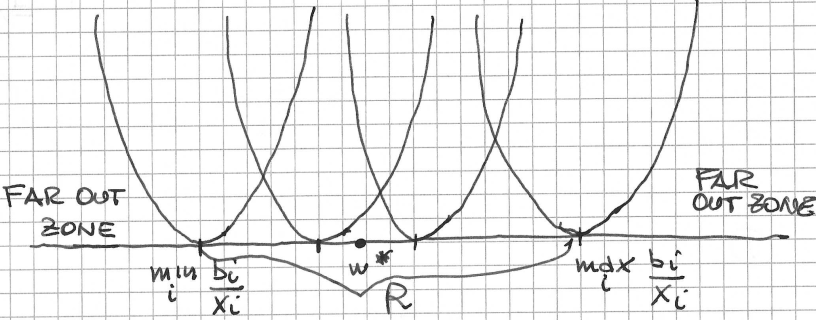
\includegraphics[scale=0.3]{../images/SGD.png}
\end{center}
Where $R$ is the Region of confusion. In the Far Out Zone (FOZ) $\nabla J_i$ has the same sign as $\nabla J$. Stochastic gradient descent uses a randomized version $g$ of $\nabla J$ and we have:
\[
    \mathbb{E}[g] = \nabla J \hspace{1cm} \text{unbiased estimator}     
\]
It is important to control the variance and speed. How to choose $i_k$:
\begin{enumerate}
    \item Randomly pick $i_k$ with replacement (good theoretically)
    \item Randomly pick $i_k$ without replacement (good in practice)
\end{enumerate}

\subsubsection{Minibatch}
It uses the following update rule:
\[
    \underline{w}^{(k+1)} = \underline{w}^{(k)} - \dfrac{\eta}{\vert I_k\vert} \sum_{j \in I_k} \nabla J_j(\underline{w}^{(k)})
\]
So, basically, we are taking the average of the gradients of the samples in the minibatch. This helps reducing the variance. Very large mini-batch shrinks confusion region (reduced noises) and can create overfitting. It helps also for parallelism. 